\section{Доменная адаптация}
\label{sec:Chapter3} \index{Chapter3}

В современном мире машинного обучения и искусственного интеллекта способность моделей адаптироваться к новым условиям и данным стала одной из ключевых задач. Традиционные методы обучения моделей предполагают, что данные, используемые для обучения и тестирования, имеют схожие характеристики и распределения. Однако в реальных приложениях часто возникает необходимость применять модели на данных, которые существенно отличаются от тех, на которых они были изначально обучены. Это приводит к снижению точности и эффективности моделей, что ставит под угрозу их практическое применение.

Для решения данной проблемы была разработана задача доменной адаптации, целью которой является создание методов для акклиматизации модели к целевым данным, отличающимся от исходных. В рамках этой задачи были разработаны подходы и техники, направленные на уменьшение расхождений между исходным и целевым доменами, что позволяет сохранять точность и производительность моделей в новых условиях. Эти методы способствуют переносу знаний, накопленных в исходном домене, на целевой, что относит данную задачу к области методов transfer learning.

\subsection{Перенос знаний}

Перенос обучения (англ. transfer learning) позволил уже существующим решениям выйти за пределы первоначально заданных задач. Этот подход позволил использовать различные архитектуры для решения новых, разнообразных проблем. К примеру, это позволило перенести опыт использования трансформеров из задач обработки естественного языка в задачи компьютерного зрения.

Помимо переноса знаний между различными областями нейронных сетей, transfer learning предоставляет возможность использовать опыт, накопленный в процессе обучения модели, для работы с новыми данными. Эти данные могут представлять собой не только новые классы в задачах классификации или кластеризации, но и иметь значительные структурные различия, такие как язык и жанр для текстовых данных или стиль и качество для изображений. Такие методы, называемые адаптацией к новым доменам данных, позволяют существенно сократить время и ресурсы, направленные на решение новых, узкоспециализированных задач.

\begin{figure}[h]
	\centering
	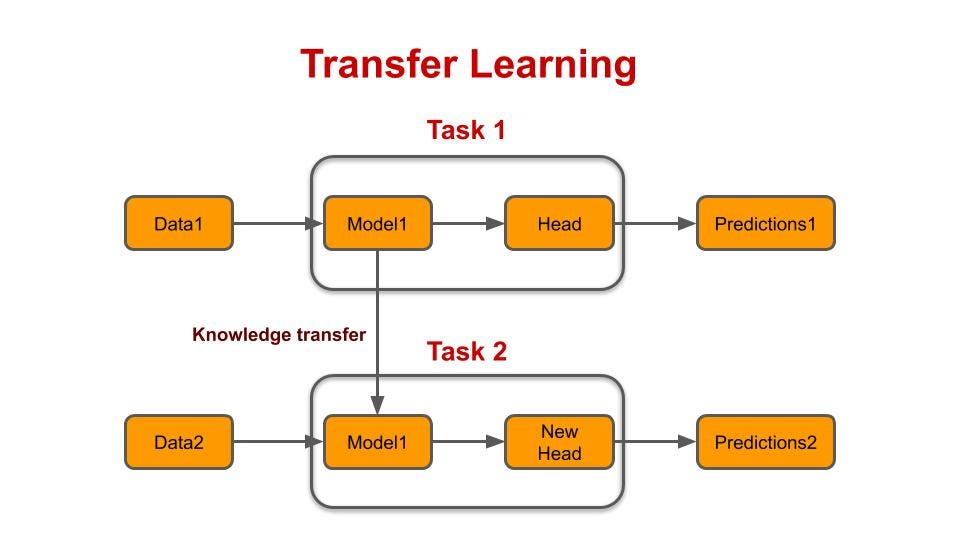
\includegraphics[width=\textwidth]{./images/TL_medium.jpg}
	\caption{Основная идея переноса знаний}
	\label{fig:tl}
\end{figure}

Основная идея состоит в том, чтобы взять модель, которая уже научилась извлекать и интерпретировать общие признаки из большого набора данных, может эффективно адаптироваться к новым данным, требующим более специфических знаний (см \autoref{fig:tl}). Это аналогично тому, как человек, обладая общими знаниями в одной области, может быстрее освоить смежную сферу деятельности. Таким образом получается не только ускорить процесс обучения, но и повысить точность и эффективность модели при условии ограниченности в ресурсах. 

\subsection{Основные определения}

Для дальнейшего повествования введем формальные обозначения для данной задачи.

\underline{Определение домена}

Пусть существует пространство признаков $\chi$ и в нем задан набор данных $X$ и частотное распределение вероятностей на нем $P(X)$:
\begin{equation}
	X = {X_1, ..., X_n} \in \chi.
\end{equation}

В таком случае \textit{доменом $D$} называют совокупность пространства признаков и частотного распределения вероятности на заданном наборе данных:
\begin{equation}
D = \{\chi, P(X)\}
\end{equation}

\underline{Определение задачи}

Пусть на пространстве признаков $\chi$ задан набор данных
\begin{equation}
	X = \{X_1, ..., X_n\} \in \chi.
\end{equation}

Пусть существует пространство меток $\gamma$ и для заданного набора данных существует соответствующий набор меток
\begin{equation}
Y = \{Y_1, ..., Y_n\} \in \gamma
\end{equation}

Тогда \textit{задача $T$} определяется как 
\begin{equation}
T = \{Y, f(X)\},
\end{equation}
где $f$ - прогностическая функция зависимости целевой переменной, которую можно рассматривать как условное вероятностное распределение $P(Y|X)$.\\

\underline{Определение доменной адаптации}

В задаче доменной адаптации подразумевается наличие не менее двух наборов данных:
\begin{enumerate}
\item \textit{Исходный домен (Source)}\\
Представляет собой универсальный набор данных большого объема. Обозначается следующим образом:
$$D^s = \{\chi^s, P(X^s)\}$$
На домене определена задача: $$T^s = \{Y^s, f^s(X^s)\}$$
\item \textit{Целевой домен (Target)}\\
Представляет собой набор данных маленького объема, к которому планируется адаптировать модель. Обозначается следующим образом:
$$D^t = \{\chi^t, P(X^t)\}$$
На домене определена задача: $$T^t = \{Y^t, f^t(X^t)\}$$
\end{enumerate}

В зависимости от того, как соотносятся между собой домены $D^S$ и $D^T$ и задачи $T^s$ и $T^t$, ставятся различные задачи:
\begin{enumerate}
\item Самым распространенным является случай совпадения задач и доменов, когда $D^s = D^t$ и $T^s = T^t$. В таком случае говорят о постановке задачи классического машинного обучения. Домен $D^s$ называют обучающей выборкой, которая используется для обучения решения $T$, а домен $D^t$ - тестовой выборкой, на которой производится оценка правильности полученного решения.

\item При совпадении данных $D^S = D^t$, но различной постановке задачи $T^s \ne T^t$ говорят о мультизадачном обучении. Часто такая постановка задачи подходит для адаптации модели классификации к новым меткам классов, которые представлены в целевой выборке, но отсутствуют в исходной.

\item При совпадении задач $T^s = T^t$, но различии в данных $D^s \ne D^t$ говорят о методах кросс-доменной адаптации. В таком случае ставится задача улучшения предсказания $T^t$ с использованием информации, полученной в $T^s$. 

\item При полном несовпадении данных $D^S \ne D^t$ и задач $T^s \ne T^t$ подразумевается, что пары $(D, T)$ решают разные проблемы и адаптация происходит в индивидуальном порядке. Например, использование архитектуры трансформер, зарекомендовавшей себя в задачах обработки естественного языка, для задач компьютерного зрения.
\end{enumerate} 

\begin{figure}[h]
	\centering
	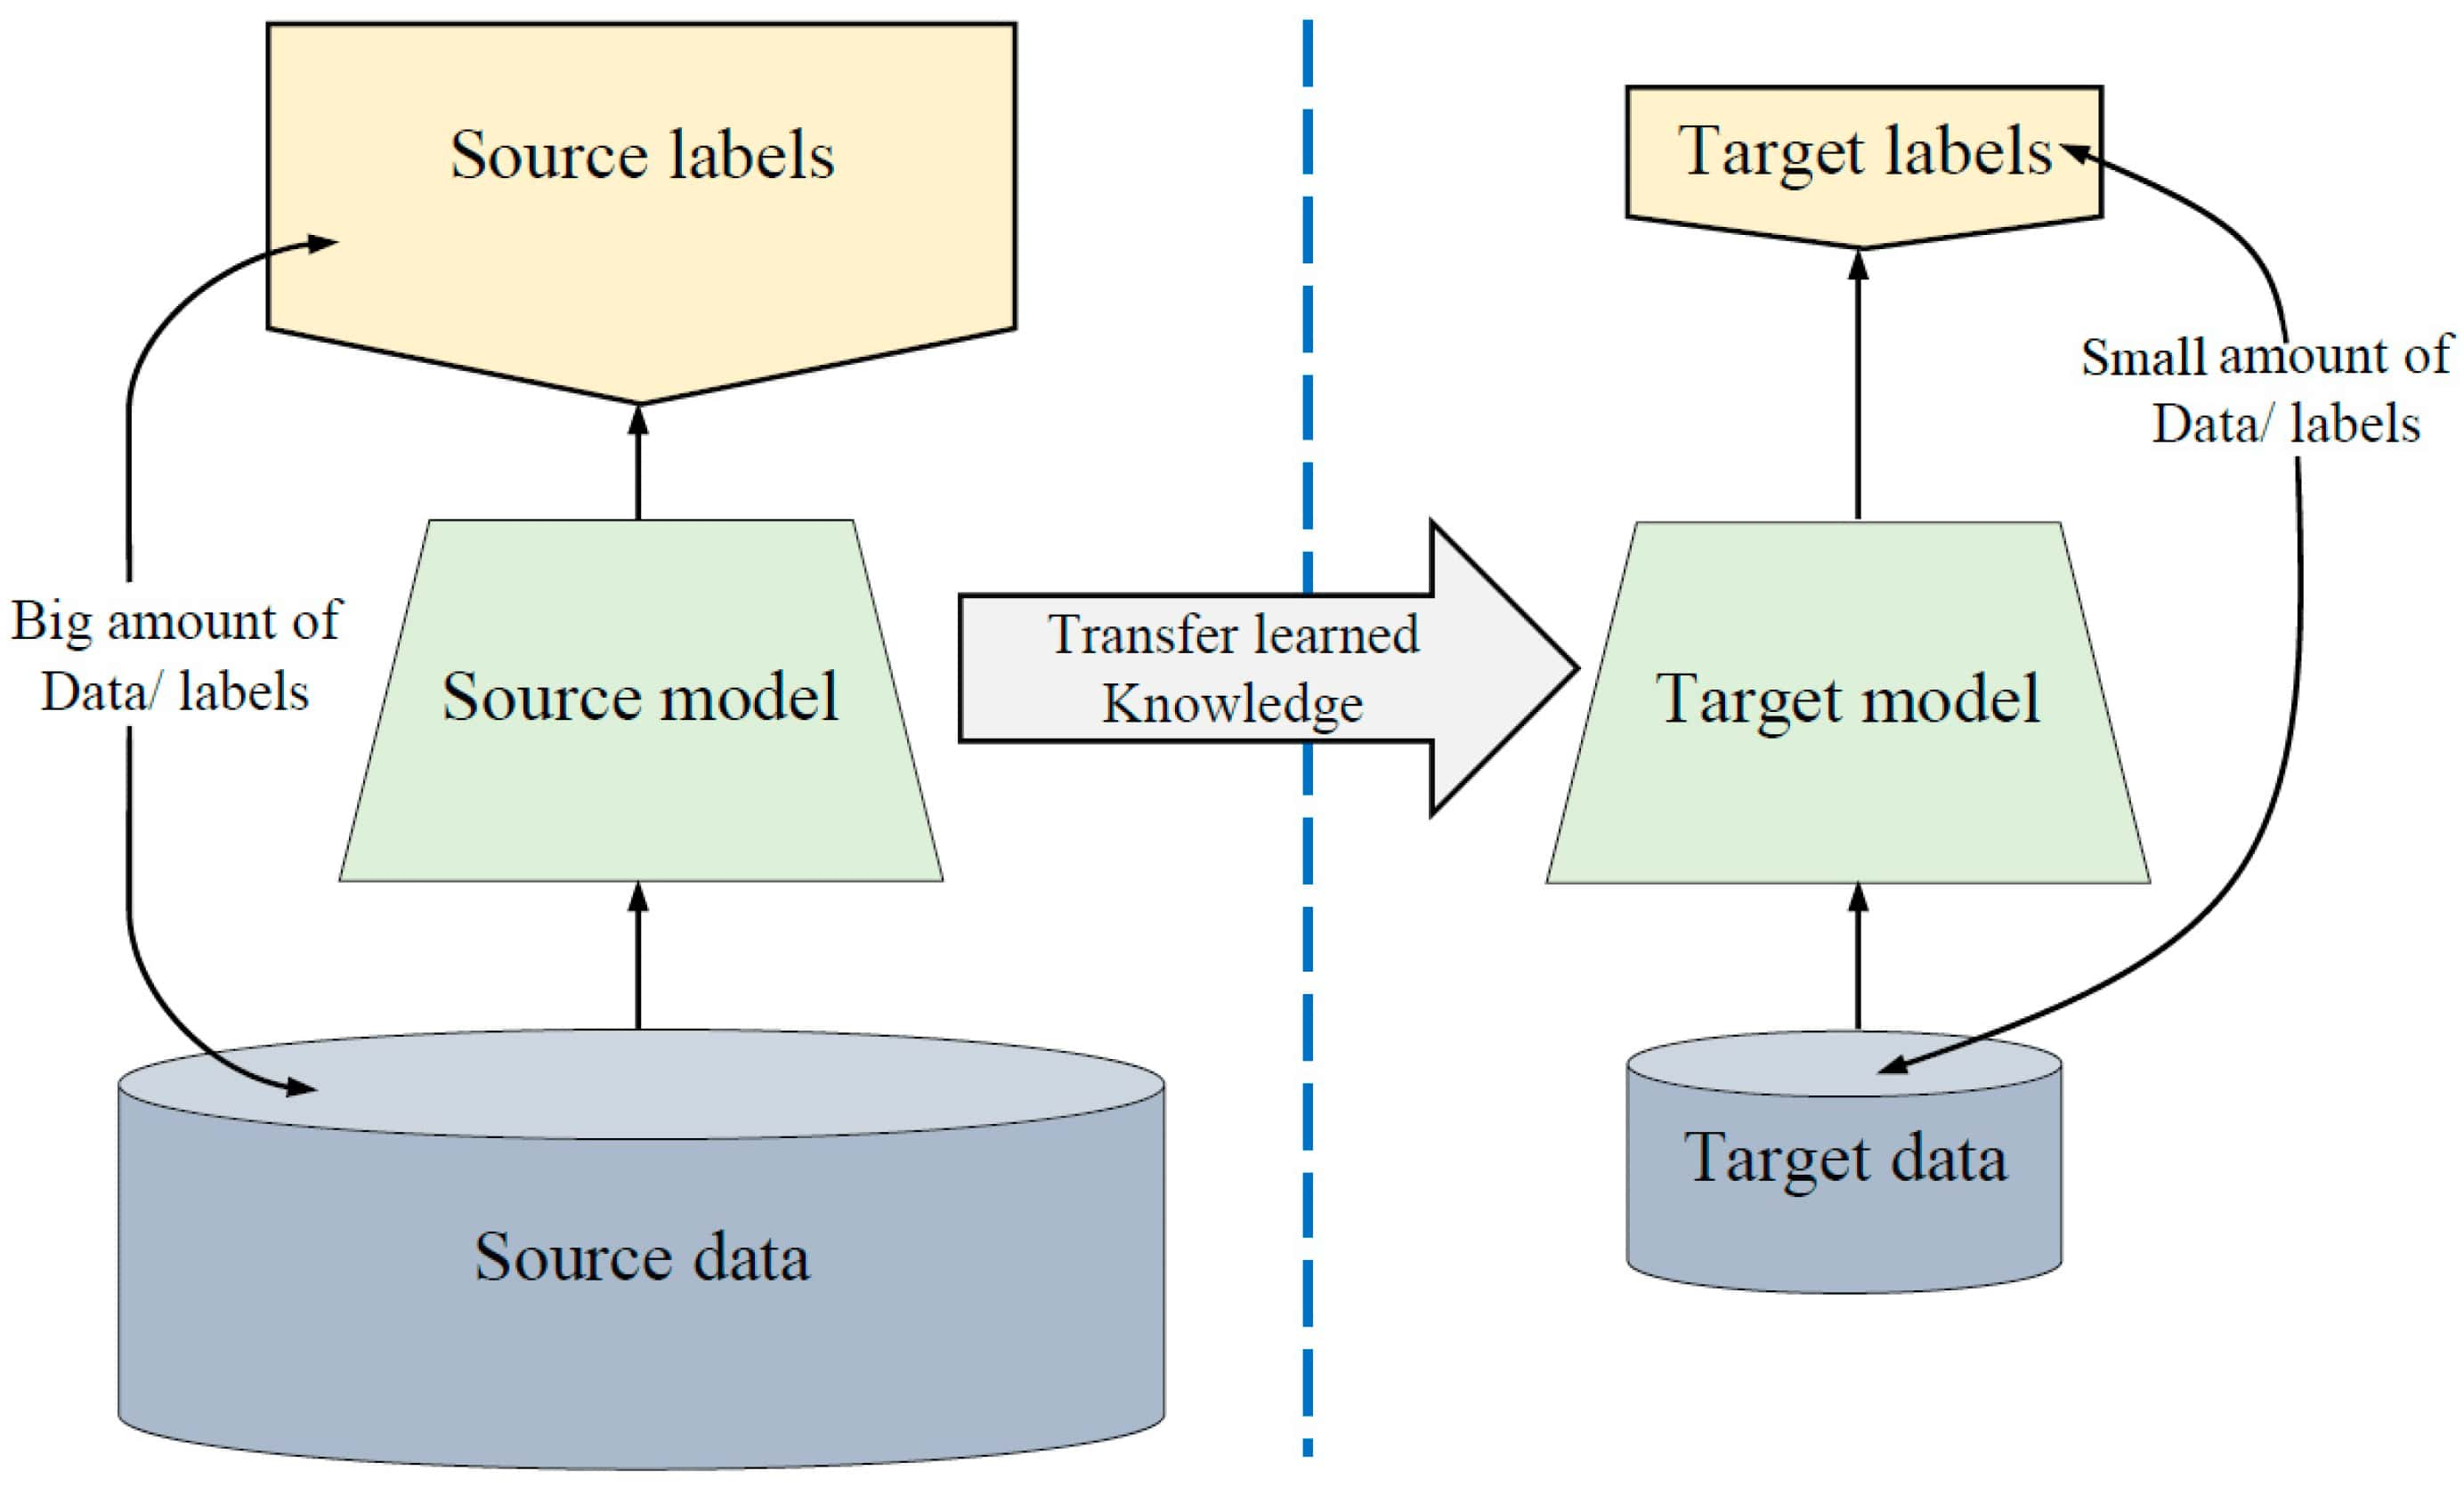
\includegraphics[width=.75\textwidth]{./images/DA.jpg}
	\caption{Схематическое представление работы алгоритмов доменной адаптации}
	\label{fig:DA}
\end{figure}

В текущей работе рассматривается третий вариант: $D^s \ne D^t$, но $T^s = T^t$. Схематически постановка задачи описана на \autoref{fig:DA}, а формулировка задачи математическим языком выглядит следующим образом:
$$D^s, T^s \to D^t, T^t$$

\subsection{Классификация методов доменной адаптации}

Ранее методы, которые решают задачу \textit{доменной адаптации (англ. domain adaptation)}  были определены как методы переноса знаний, направленные на на приспособление моделей $T^s = T^t = T$, обученных на данных из домена $D^s$, к данным из домена $D^t$, причем $D^s \ne D^t$. Данные могут различаться по различным характеристикам и в зависимости от различают несколько типов методов, которые схематически представлены на \autoref{fig:DA_classification}.

\begin{figure}[h]
	\centering
	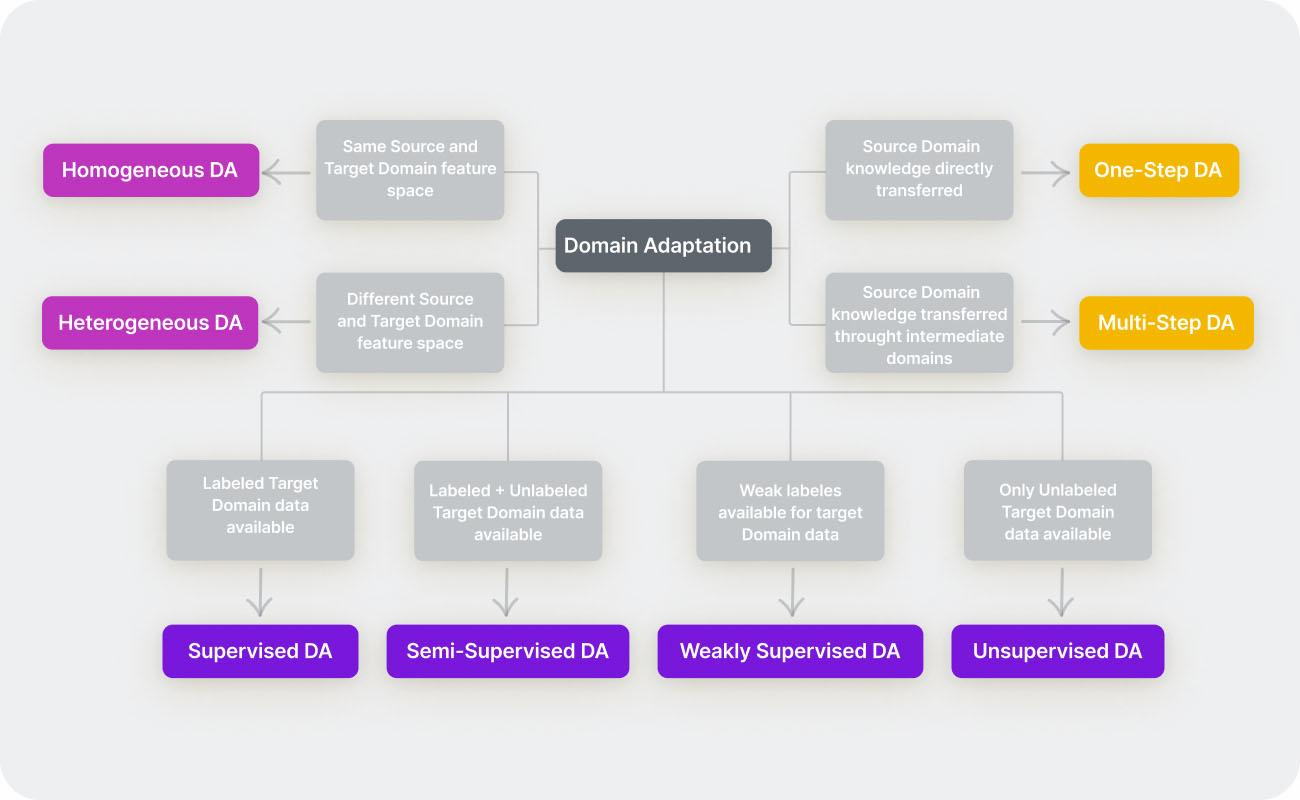
\includegraphics[width=.9\textwidth]{./images/DA_classification.jpg}
	\caption{Схематическое представление работы алгоритмов доменной адаптации}
	\label{fig:DA_classification}
\end{figure}

\hfill \break
В зависимости от того, насколько сопоставляются распределения наборов данных $P(X)$ различают гомогенные и гетерогенные методы.

\begin{enumerate}
\item \textit{Гомогенные методы (Homogeneous DA)}

Данный тип методов применяется, когда исходный и целевой домены имеют одинаковое пространство признаков $\chi^s = \chi^t = \chi$, но их распределения отличаются $P(X^s) \ne P(X^t)$. Методы гомогенной адаптации фокусируются на выравнивании распределений признаков между доменами, чтобы модель, обученная на исходных данных $D^s$ , могла эффективно работать на целевых данных $D^t$.

\item \textit{Гетерогенные методы (Heterogeneous DA)}

В отличие от предыдущих способов, в текущем случае отличаются и признаковые пространства между доменами $\chi^s \ne \chi^t$. Это представляет собой более сложный сценарий, так как необходимо либо преобразовывать целевые данные в такое представление, которое будет сопоставимо с исходными, либо выуживать обобщенные признаки из обоих доменов, на которых модель будет считать данные похожими.

\end{enumerate}

\hfill \break
Также стоит обратить внимание насколько сильно отличаются распределения данных, так как от этого зависит сколько шагов необходимо будет производить между доменами:

\begin{enumerate}
\item \textit{Одношаговая доменная адаптация (One-step DA)}

При небольших различиях между распределениями можно использовать прямой перенос знаний из $D^s$ в $D^t$. В таком случае опыт, накопленный моделью в исходном домене, напрямую используется при адаптации модели $T$ на целевом домене. Преимущества этого метода заключаются в его простоте и быстроте внедрения, так как он не требует промежуточных шагов.

\item \textit{Многошаговая доменная адаптация (Multi-step DA)}

Однако эффективность One-Step DA может снижаться, когда различия между исходным и целевым доменами слишком велики для прямого переноса знаний. Для этих случаев и используются методы многошаговой адаптации. Они подразумевают поэтапное выполнение: знания из исходного домена сначала переносятся в один или несколько промежуточных доменов, прежде чем достигнуть целевого. Промежуточные шаги помогают постепенному выравниванию распределения данных, что улучшает адаптацию и повышает точность модели в целевом домене.

\end{enumerate}

\hfill \break
Последним маркером в классификации методов доменной адаптации является доступность размеченных данных для $D^t$. По данному признаку методы разделяются сразу на 4 группы:

\begin{enumerate}
\item \textit{Supervised domain adaptation}

В этом случае обучение модели происходит с использованием как исходных, так и целевых данных, имеющих метки. Поэтому данные методы обычно достигают высокой точности, поскольку модель может явно учиться на целевых данных с метками.

\item \textit{Semi-supervised domain adaptation}

К данным методам прибегают, когда в целевом домене присутствуют как размеченные данные, которые используются для начального обучения, так и неразмеченные данные, на которых есть возможность улучшать работу модели. 

\item \textit{Weakly supervised domain adaptation}

Когда данные целевого домена слабо размечены, то есть использовалась автоматическая система разметки, которая допускает ошибки, используются методы weakly supervised DA. Они направлены либо на улучшение точности слабых меток, либо используют <<мягкие>> техники регуляризации, что позволяет учитывать возможность ошибки в данных.


\item \textit{Unsupervised domain adaptation}

Самый сложный случай, когда нет возможности аннотировать домен и надо на сырых данных улучшить качество модели. Для методов этого типа часто используется кластеризация данных и итеративные подходы, которые помогают модели $T$ улучшать собственные предсказания.

\end{enumerate}


\newpage